
\begin{exerciseS}[Metodo di Pistolesi]
Il metodo di Pistolesi è un primo metodo rudimentale per la modellazione di profili
bidimensionali nell'ambito della teoria a potenziale. Il profilo viene approssimato con una lamina piana. 
L'effetto del profilo viene modellato tramite la sovrapposizione a una corrente asintotica di un vortice posto a un quarto di corda (corrispondente all'incirca con la posizione del centro aerodinamico - def...). Il valore della circolazione (e quindi della portanza) viene ricavato imponendo le condizioni al contorno in un punto di controllo sul profilo.

Assumendo sia valida l'approssimazione per piccoli angoli $\sin \alpha \sim \alpha$, confrontando la formula della portanza $l = \frac{1}{2} \rho U^2 c c_L$ con quella ottenuta dal teorema di Kutta-Joukowski, ipotizzando un valore di $c_{L_\alpha} = 2\pi$,
si trovi il punto di controllo nel quale deve essere imposta la condizione al contorno.

Quale condizione al contorno va imposta e perchè?
\end{exerciseS}


\sol

\partone Metodi a pannelli. Metodo di Pistolesi. Aerodinamica potenziale.
  
\parttwo
La condizione da imporre è quella di tangenza: la velocità nel punto di controllo deve essere tangente alla lamina piana.

Definita $b$ la distanza del punto di controllo dal centro aerodinamico, si impone la condizione al contorno in tale punto: deve essere nulla la componente normale alla lamina della velocità ottenuta come sovrapposizione della corrente asintotica e della corrente indotta dal vortice.

\begin{equation}
  0 = \frac{\Gamma}{2\pi b} + U_\infty \sin \alpha \qquad \Rightarrow \qquad 
  \Gamma = - 2\pi b U_\infty \alpha
\end{equation}

Inserita nel teorema di Kutta-Joukowski  $l = -\rho \Gamma U_\infty = \rho U_\infty^2 b 2\pi \alpha$ e confrontata alla formula della portanza $l = \frac{1}{2} \rho U^2 c c_L$, si ottiene

\begin{equation}
  b = \frac{c}{2}
\end{equation}

Quindi nel metodo di Pistolesi, il centro aerodinamico è posizionato $\frac{1}{4}$  di corda, mentre il punto di controllo è posizionato a $\frac{3}{4}$ di corda.

\vspace{0.5cm}
\textit{Osservazioni.} 
\begin{itemize}

\item \'E possibile simulare l'interazione tra più profili. Con metodi a pannelli un po' più raffinati
   (Hess Smith, Morino,...) è possibile simulare l'interazione tra corpi aerodinamici di forma qualsiasi,
   ricordandosi che le informazioni ottenute sono valide sotto le ipotesi dell'aerodinamica a potenziale:
   non devono verificarsi grandi separazioni, la vorticità deve essere confinata in una regione sottile
   (numero di Reynolds elevato).
  

\item Quale può essere un metodo per simulare l'effetto di una superficie piana infinita (effetto suolo)?

\end{itemize}

\newpage
\clearpage

\begin{exerciseS}[Effetto suolo e interazione profili]
Usare il metodo di Pistolesi per ottenere delle informazioni qualitative sul coefficiente
 di portanza
\begin{itemize}
 \item di un profilo in effetto suolo 
 \item di due profili, in funzione della posizione reciproca
\end{itemize}
\end{exerciseS}

\paragraph{Confronto con i risultati ottenuti con il metodo di Hess Smith:
 effetto suolo.}
Con il metodo delle immagini è possibile calcolare l'effetto che ha la
 presenza di una parete orizzontale (parallela alla velocità asintotica)
 sul coefficiente di portanza di un profilo NACA2412 con incidenza 
 $\theta = 2\degree$. Il coefficiente di portanza in ``aria libera'' è
 $c_{L0} = 0.481$. La distanza del profilo dalla parete è adimensionalizzata
 sulla corda.

\begin{tabular}{cc}
\begin{minipage}{0.47\textwidth}
\begin{verbatim}
  h/c      cL     DcL/cL0
-----------------------------
 0.500   0.680     0.261
 1.000   0.536     0.112
 1.500   0.508     0.054
 2.000   0.498     0.033
 2.500   0.493     0.022
 3.000   0.490     0.016
 3.500   0.488     0.012
\end{verbatim}
\end{minipage}
&
\begin{minipage}{0.47\textwidth}
\begin{center}
\begin{tikzpicture}
\begin{axis}[axis x line=bottom, axis y line=middle, domain=-1.2:3.2, xlabel={$c_L/c_{L0}$}, ylabel={$h/c$},xmin=1.0,xmax=1.5,ymin=0.0,ymax=3.5]
\addplot coordinates{
(  1.261 ,  0.500  ) 
(  1.112 ,  1.000  ) 
(  1.054 ,  1.500  ) 
(  1.033 ,  2.000  ) 
(  1.022 ,  2.500  ) 
(  1.016 ,  3.000  ) 
(  1.012 ,  3.500  ) 
};
\legend{$c_L/c_{L0}$}
\end{axis}
\end{tikzpicture}
\end{center}
\end{minipage}
\end{tabular}

\paragraph{Confronto con i risultati ottenuti con il metodo di Hess Smith:
 due profili.} Quando due profili sono investiti da una corrente, ognuno
 di essi influenza l'altro. Come primo esempio vengono usati due profili
 NACA0012, con la stessa corda. Il secondo profilo viene messo in scia al
 primo a distanza di 3 corde. La prima prova consiste nel mantenere il 
 secondo profilo a incidenza nulla rispetto alla velocità asintotica, 
 aumentando l'incidenza del primo. Il primo profilo genera una portanza
 inferiore a un profilo in aria libera, mentre il secondo è deportante: il
 primo profilo induce una velocità verso il basso sul profilo in coda, che
 quindi vede un'incidenza non nulla, ma negativa.
\begin{center}
\begin{verbatim}
 theta2 = 0.0\degree
-------------------------------
 theta1    cL1     cL2    cL10 
-------------------------------
   2.5°  0.286  -0.045   0.297 
   5.0°  0.571  -0.089   0.594 
\end{verbatim}
\end{center}

 La seconda prova consiste nel mantenere il primo profilo a incidenza nulla
 rispetto alla velocità asintotica e aumentare l'incidenza del profilo in scia.
 Il secondo profilo ha un coefficiente di portanza minore rispetto a quello
 di un profilo in aria libera; il primo profilo è anch'esso portante: il
 profilo in scia induce una velocità verso l'alto sul primo profilo che quindi
 vede un'indicenza positiva.
\begin{center}
\begin{verbatim}
 theta1 = 0.0°
-------------------------------
 theta2    cL1     cL2    cL20 
-------------------------------
   2.5°  0.064   0.287   0.297 
   5.0°  0.128   0.573   0.594 
\end{verbatim}
\end{center}
 La portanza risultante è maggiore a quella che si otterrebbe considerando
 la somma della portanza generata singolarmente dai due profili. Per esempio,
 per $\theta = 2.5°$:
\begin{equation}
\begin{aligned}
 c_{L1} + c_{L2} & > c_{L01} + c_{L02} \\
  0.064 + 0.287  & >  0.000  +  0.297  \\
          0.351  & >  0.297
\end{aligned}
\end{equation}
Lo stesso effetto viene osservato con due profili più vicini tra loro. La corda
 del profilo secondario è la metà di quella del profilo principale.
 Il profilo principale ha incidenza $\theta_1 = -0.5°$ rispetto alla velocità
 asintotica, quello secondario $\theta_2 = 12°$. La presenza del secondo 
 profilo fa aumentare significativamente la portanza del profilo principale.

\begin{tabular}{ll}
\begin{minipage}{0.43\textwidth}
\begin{center}
\begin{verbatim}
          +------------------------
          | theta  |   cL  |  cL0 
----------+--------+-------+-------
airfoil 1 |  -0.5° | 1.099 | 0.184
airfoil 2 |  12.0° | 0.975 | 1.656
----------+--------+-------+-------
\end{verbatim}
\end{center}
La colonna $\mathtt{cL}$ contiene i coefficienti di portanza dei profili
 disposti
 come in figura. La colonna $\mathtt{cL0}$ contiene i coefficienti di portanza
 dei
 profili presi singolarmente, senza influenza reciproca, alla stessa incidenza.
%  Per ottenere la portanza complessiva, bisogna ricordarsi che i coefficienti
%  dei due profili sono adimensionalizzati sulle rispettive corde.
 
%  -----------------------
%    cL20  theta2    cL2  
%  -----------------------
%    1.656  12.0°   0.975 
\end{minipage}
&
\begin{minipage}{0.57\textwidth}
\begin{center}
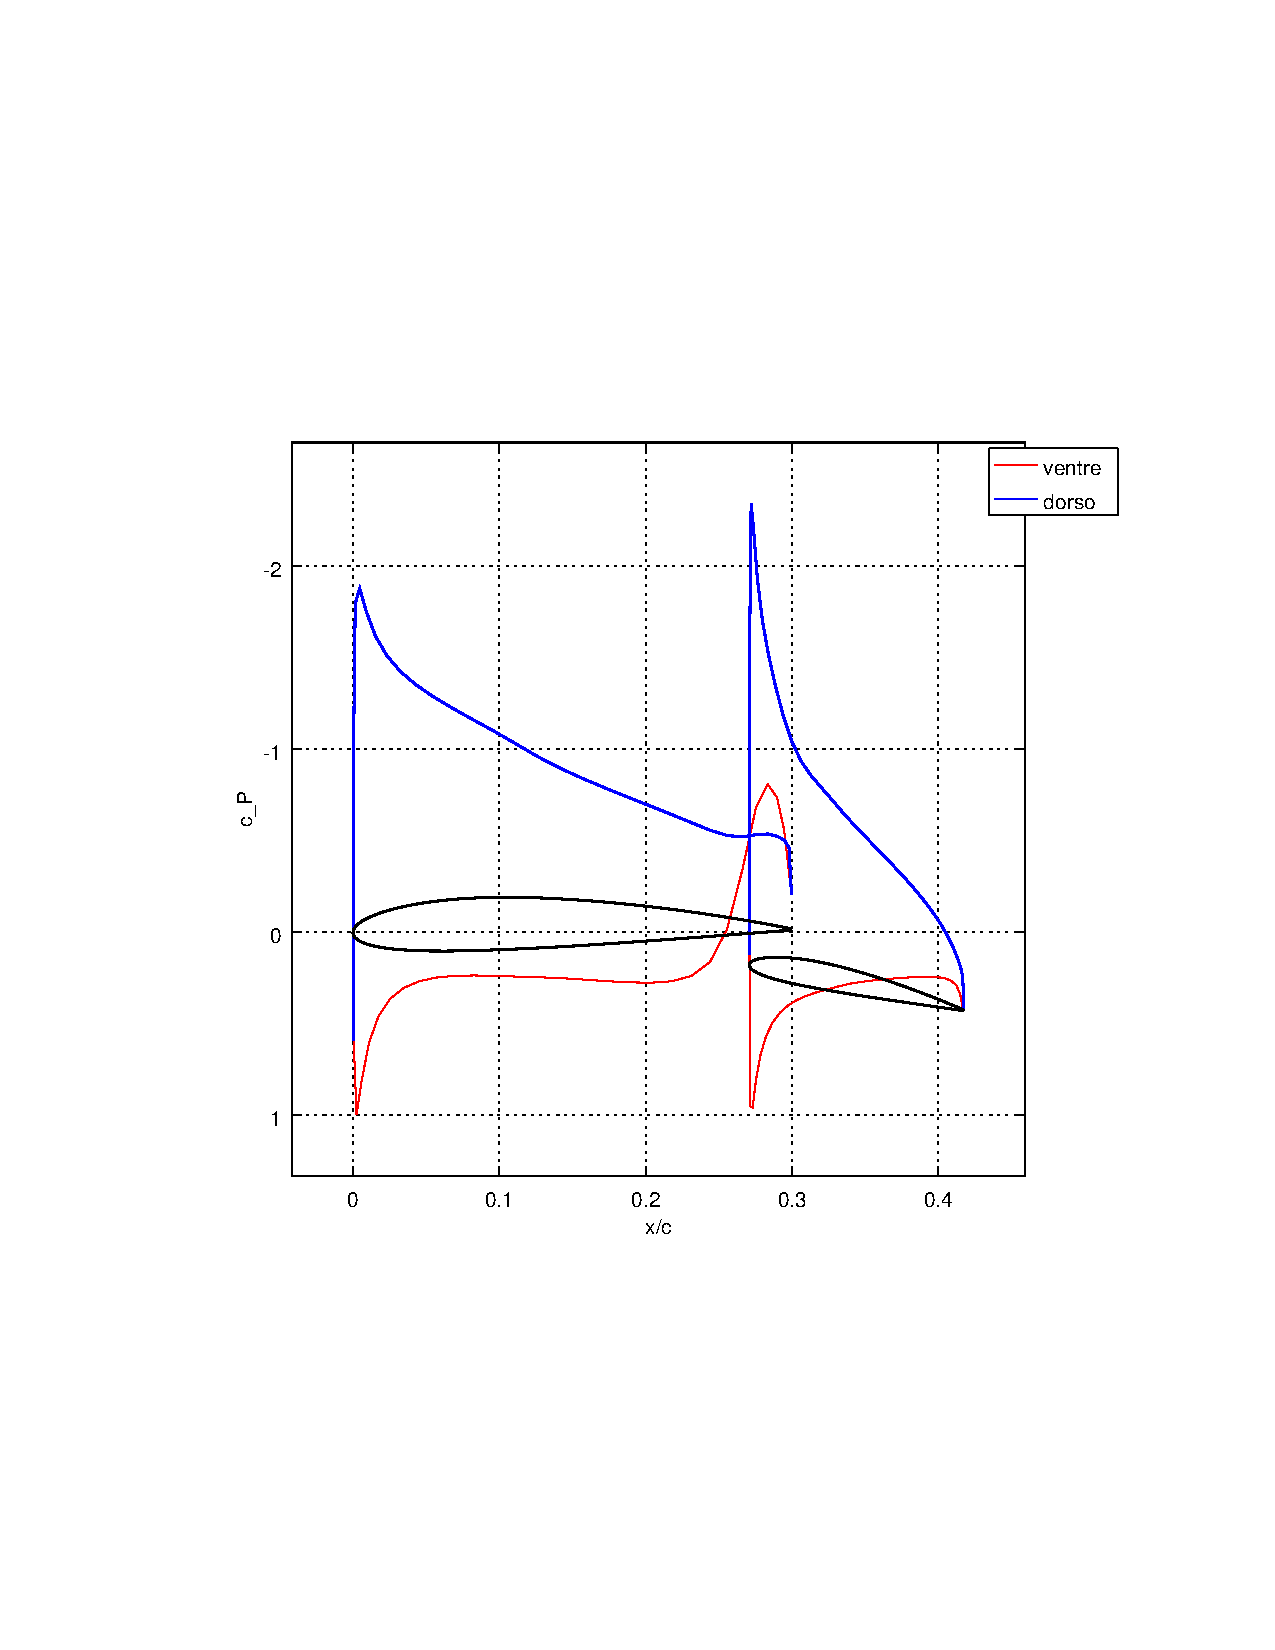
\includegraphics[width=0.95\textwidth,trim={3cm 6cm 2cm 6cm},clip]
        {./fig/Aileron.pdf}
\end{center}
\end{minipage}
\end{tabular}

Come ultimo esempio si considerano due profili NACA0012 uguali sovrapposti,
 con angolo di incidenza $\theta=5.0°$, separati da una distanza
 adimensionalizzata $y/c$ compresa tra 1 e 15. Il coefficiente di portanza
 del singolo profilo è $c_L = 0.594$.

\begin{center}
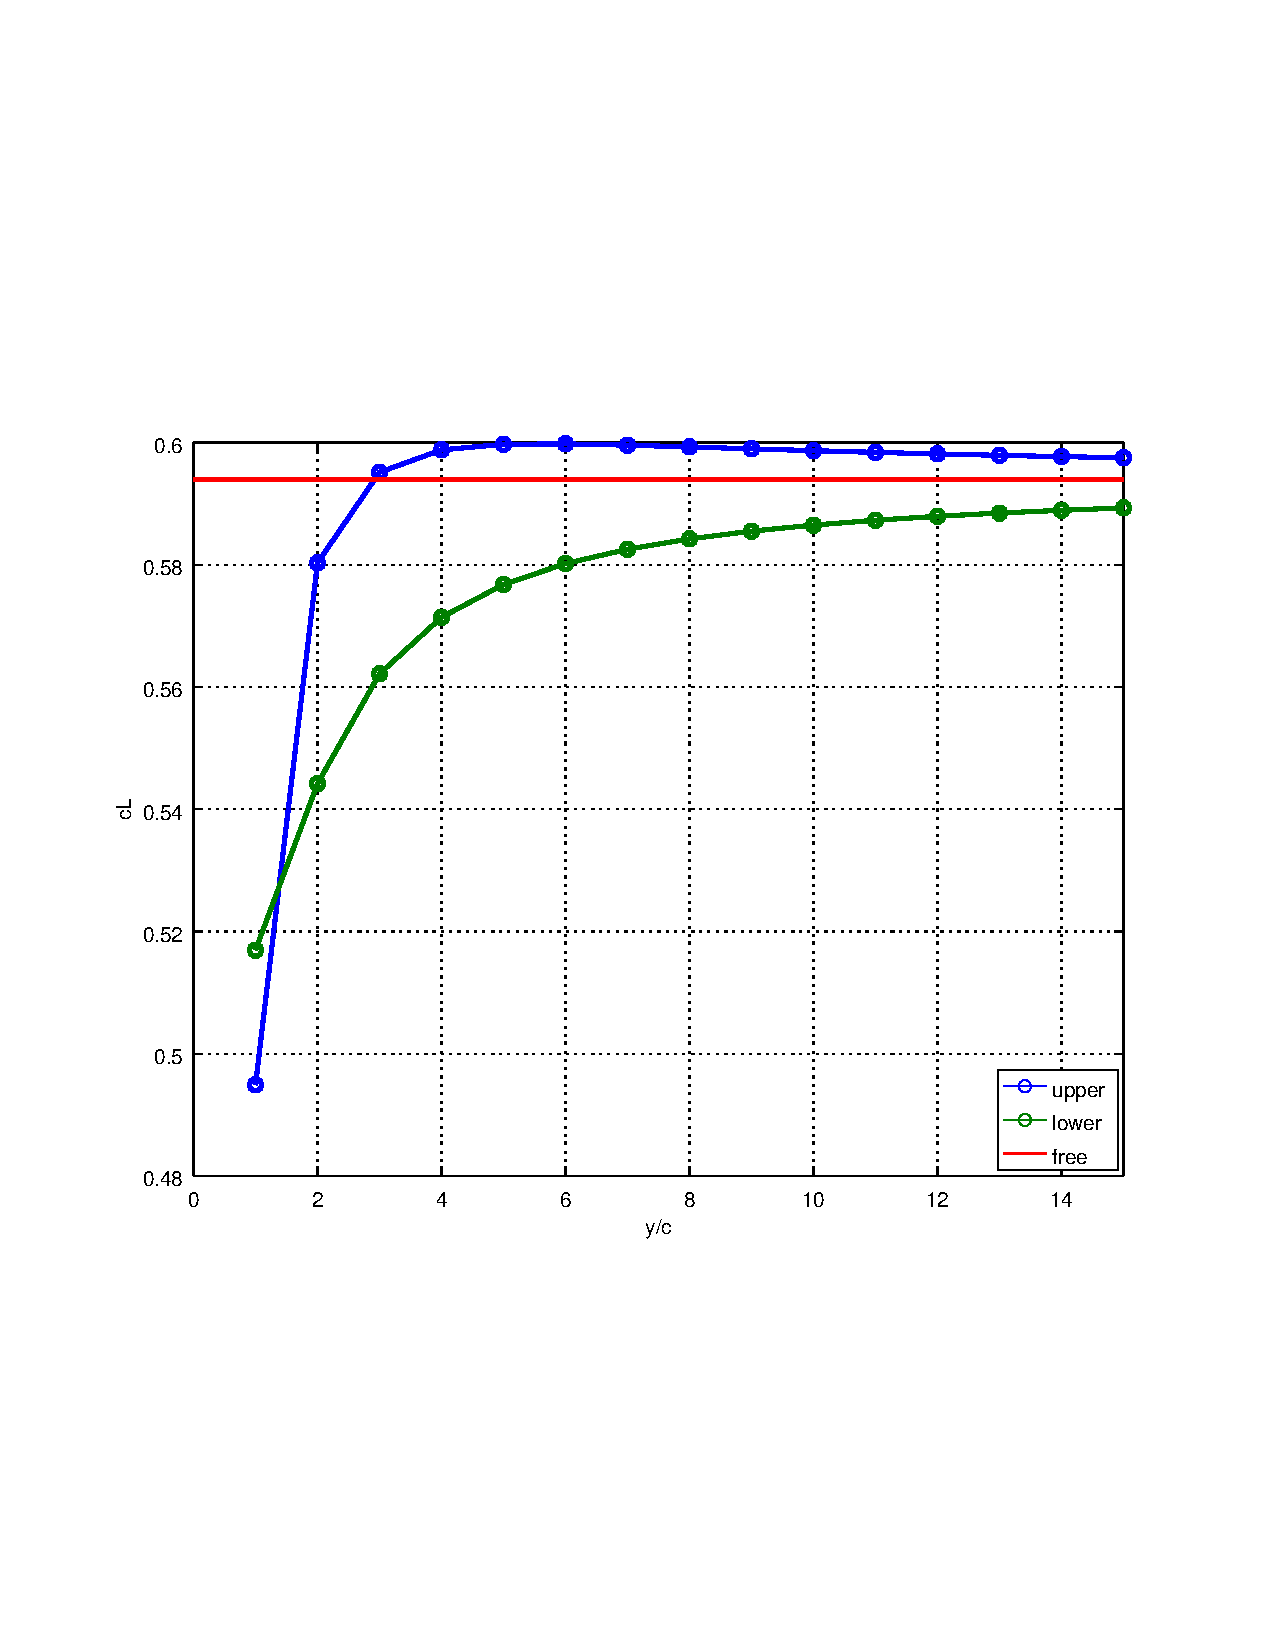
\includegraphics[width=0.60\textwidth,trim={0 5cm 0 5cm},clip]
       {./fig/vanes.pdf}
\end{center}

\noindent
Esistono alcuni esempi "esotici": ekranoplano sovietico...; esempi meno esotici:...
